\let\negmedspace\undefined
\let\negthickspace\undefined
\documentclass[journal]{IEEEtran}
\usepackage[a5paper, margin=10mm, onecolumn]{geometry}
\usepackage{tfrupee} 
\setlength{\headheight}{1cm} 
\setlength{\headsep}{0mm}     

\usepackage{gvv-book}
\usepackage{gvv}
\usepackage{cite}
\usepackage{amsmath,amssymb,amsfonts,amsthm}
\usepackage{algorithmic}
\usepackage{graphicx}
\usepackage{textcomp}
\usepackage{xcolor}
\usepackage{txfonts}
\usepackage{listings}
\usepackage{enumitem}
\usepackage{mathtools}
\usepackage{gensymb}
%\usepackage{wasysym}
\usepackage{comment}
\usepackage[breaklinks=true]{hyperref}
\usepackage{tkz-euclide} 
\usepackage{listings}
\def\inputGnumericTable{}                                 
\usepackage[latin1]{inputenc}                                
\usepackage{color}                                            
\usepackage{array}                                            
\usepackage{longtable}                                       
\usepackage{calc}                                             
\usepackage{multirow}                                         
\usepackage{hhline}                                           
\usepackage{ifthen}                                           
\usepackage{lscape}
\usepackage{circuitikz}
\tikzstyle{block} = [rectangle, draw, fill=blue!20, 
    text width=4em, text centered, rounded corners, minimum height=3em]
\tikzstyle{sum} = [draw, fill=blue!10, circle, minimum size=1cm, node distance=1.5cm]
\tikzstyle{input} = [coordinate]
\tikzstyle{output} = [coordinate]
\renewcommand{\thefigure}{\theenumi}
\renewcommand{\thetable}{\theenumi}
\setlength{\intextsep}{10pt} % Space between text and floats
\numberwithin{equation}{enumi}
\numberwithin{figure}{enumi}
\renewcommand{\thetable}{\theenumi}

\begin{document}

\bibliographystyle{IEEEtran}
\vspace{3cm}

\title{7.4.39}
\author{EE25BTECH11032 - Kartik Lahoti}
\maketitle

\subsection*{Question: } 

If $\brak{m_i , \frac{1}{m_i}}$ , $m_i > 0 , i = 1, 2,3,4$ are four distinct points on a circle, then show that $m_1m_2m_3m_4 = 1 $

\textbf{Solution}:\\


Let the circle equation be 
\begin{align}
    \norm{\vec{x}}^2 + 2\vec{u}^{\top}\vec{x} + f = 0 
\end{align}

where, $\vec{u} = \myvec{a \\ b}$ with $a$ and $b$ as constants.

Let $\vec{P} = \myvec{m \\ \frac{1}{m}}$ be a arbitrary vector in space.

Putting $\vec{P}$ in the circle , we get 


\begin{align}
    \norm{\vec{P}}^2 + 2\vec{u}^{\top}\vec{P} + f = 0 
\end{align}

\begin{align}
    m^2 + \frac{1}{m^2} + 2am + \frac{2b}{m} + f = 0
\end{align}
Let, 
\begin{align}
    p\brak{m} = m^4 + 2am^3 + fm^2 + 2bm + 1 = 0 \label{eq_1}
\end{align}

A general polynomial of degree $n$, has companion matrix as

\begin{align}
   \vec{C} = \myvec{0 & 0 & 0 & \cdots & 0 & -c_{0} \\
1 & 0 & 0 & \cdots & 0 & -c_{1} \\
0 & 1 & 0 & \cdots & 0 & -c_{2} \\
0 & 0 & 1 & \cdots & 0 & -c_{3} \\
\vdots & \vdots & \vdots & \ddots & \vdots & \vdots \\
0 & 0 & 0 & \cdots & 1 & -c_{n-1}}
\end{align}

The eigen values of the Companion Matrix $\vec{C}$ are the roots of the polynomial.

For the question , 
\begin{align}
    \vec{C} = \myvec{0&0&0&-1\\
                     1&0&0&-2b\\
                     0&1&0&-f\\
                     0&0&1&-2a}\\ 
    \mydet{m\vec{I}- \vec{C}} = p\brak{m}
\end{align}

Here Eigen values of $\vec{C}$ are $m_i$ where $i \in \cbrak{1,2,3,4}$

Introducing Reversal Matrix 
\begin{align}
    \vec{J} &= \myvec{0&0&0&1\\0&0&1&0\\0&1&0&0\\1&0&0&0} \\ 
    \vec{J}^2 &= \vec{I} \label{eq_2}
\end{align}

The Matrix $\vec{J}$ flips Rows when pre-multiplied and flips column when post-multiplied.

Then,

\begin{align}
    \mydet{\frac{1}{m}\vec{I}-\vec{J}\vec{C}\vec{J}} = p\brak{\frac{1}{m}}
\end{align}

Since $p\brak{\frac{1}{m}}$ has eigen values $1/m_i$ , we can say 
\begin{align}
    \vec{J}\vec{C}\vec{J} = \vec{C}^{-1} \\
\end{align}

Taking determinant, using \ref{eq_2}

\begin{align}
    \mydet{\vec{C}} &= \mydet{\vec{C}^{-1}}\\
    \mydet{\vec{C}}^2 &= 1 
\end{align}

Since $\vec{C}$ is a real companion matrix of a monic quartic whose constant term is $1$ , 

\begin{align}
    \mydet{\vec{C}} &= \brak{-1}^4 1 
\end{align}

Also, 
\begin{align}
    \mydet{\vec{C}} &= m_1m_2m_3m_4
\end{align}

\begin{align}
    \therefore m_1m_2m_3m_4 &= 1 
\end{align}

Hence Proved

 \begin{figure}[H]
     \centering
     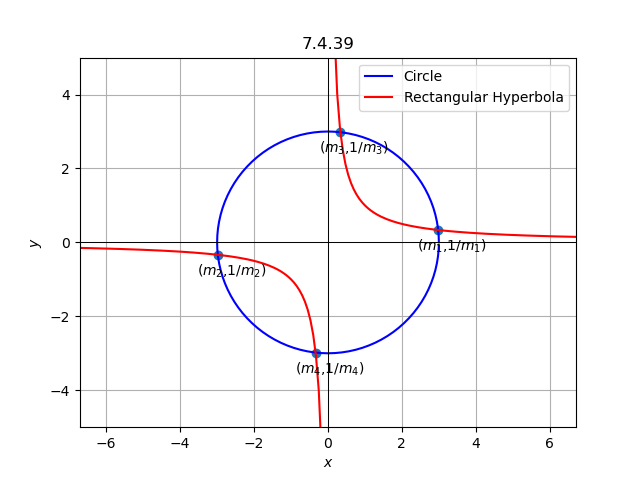
\includegraphics[width=1.0\columnwidth]{figs/graph1.png}
     \caption*{}
     \label{fig:placeholder}
 \end{figure}

\end{document}


% \begin{align}
%     a_0x^n + a_1x^{n-1} + a_2x^{n-2} \dots + a_nx^0 = 0  
% \end{align}

% Product of roots is given by 
% \begin{align}
%     \brak{-1}^n\frac{a_n}{a_0}
% \end{align}

% Since , $m_i , $ where $ i \in \cbrak{1,2,3,4} $ satisfies the equation \ref{eq_1}.
